\section{Discussion and results}

Both fjord models are run twice. The first run use the original tidal forcing, as generated directly from the TPXO atlases, and the second run with the adjusted tidal forcing. The results improved for both the Oslofjord, and for the Saltstraum. The results for the Oslofjord can be viewed in Table \ref{tab:Viker} \& \ref{tab:Oscarsborg}. In Table \ref{tab:Viker} we show that the adjustment has the desired effect close to the open boundary, while Table \ref{tab:Oscarsborg} shows that the simulated tides are distributed as intended in the inner parts of the fjord. For the Salstraum, Table \ref{tab:Bodo} shows that the amplitudes are still too small in the second run, but closer to the observed values than the first run. The error in phase for M$_2$ was only $0.8$ degrees which corresponds to three minutes (Table \ref{tab:Bodo}).

The barotropic tide propagates with a phase speed of $c = \omega/k \approx \sqrt{g h_c}$ where $g$ is the acceleration of gravity and $h_c$ is the characteristic depth. The distance from Viker to Oscarsborg is approximately 75 km and the mean depth is around 200 meters which gives an approximate phase speed of 44 m/s and a phase lag of approximately 28 minutes. According to Table \ref{tab:Viker} and \ref{tab:Oscarsborg} the observed phase lag is 17 degrees for M$_2$ which corresponds to 35 minutes which is only slightly longer than the approximate theoretical phase lag. 

Fields of the amplitude and phase for M$_2$ in the Oslofjord reveal some interesting phenomenas (Figure \ref{fig:Oslofjord_tidal_fields}). The M$_2$ amplitude decreases gradually northward from the open boundary in the south.  In the western branch the amplitude decreases as the water pass through the very narrow passage called Svelvikstraumen, while the amplitude increases north of the sill in the eastern branch. The M$_2$ phase decreases in the eastern branch, but increases in the western branch. The observed phase delay is more pronounced in the observations than in the model. The cause is most probably the smoothing of the topography in the model.

The spatial variation is larger in the Saltstraum model. Outside the Saltstraum, the narrow straight separating the two fjords, the M$_2$ amplitude is quite uniformly at approximately $80$ cm, while on the inside it is only about $35$ cm. The corresponding phase delay is approximately $60$ degrees. Unfortunately, there is no availale tidal gauges inside of the Saltstraum.
%, so we have no means of validating whether or not these values are correct. But we can speculate that we would se similar inconsistencies as those in the Oslofjord, due to smoothing of the model topography.


%The Saltstraumen is one of the worlds strongest tidal currents. Due to a narrow passage the tidal amplitude is much smaller inside the narrow passage than outside the passage, resulting in strong currents. 
%The presence of Saltstraumen as a major impact on the circulation in the Saltfjord. According to \cite{svendsen96} an anticyclonic vortex is formed to the northeast of Saltstraumen, and a cyclonic vortex to the northwest.
%%% Fra Svendsen et. al 1996
%%%They are caused by the high velocity water coming out from Saltstraumen on the falling tide, where the velocity reaches a maximum of about 4 m s1: The anti-cyclonic vortex is weaker when the tide is rising, but does not reverse direction. The cyclonic vortex almost vanishes on rising tides. These results are in accordance with the results from Resipientunderskelse (Anon., 1990) where a direct measurement of the velocity field was performed over a time period of 10 days.


\begin{figure}[!t]
\centering
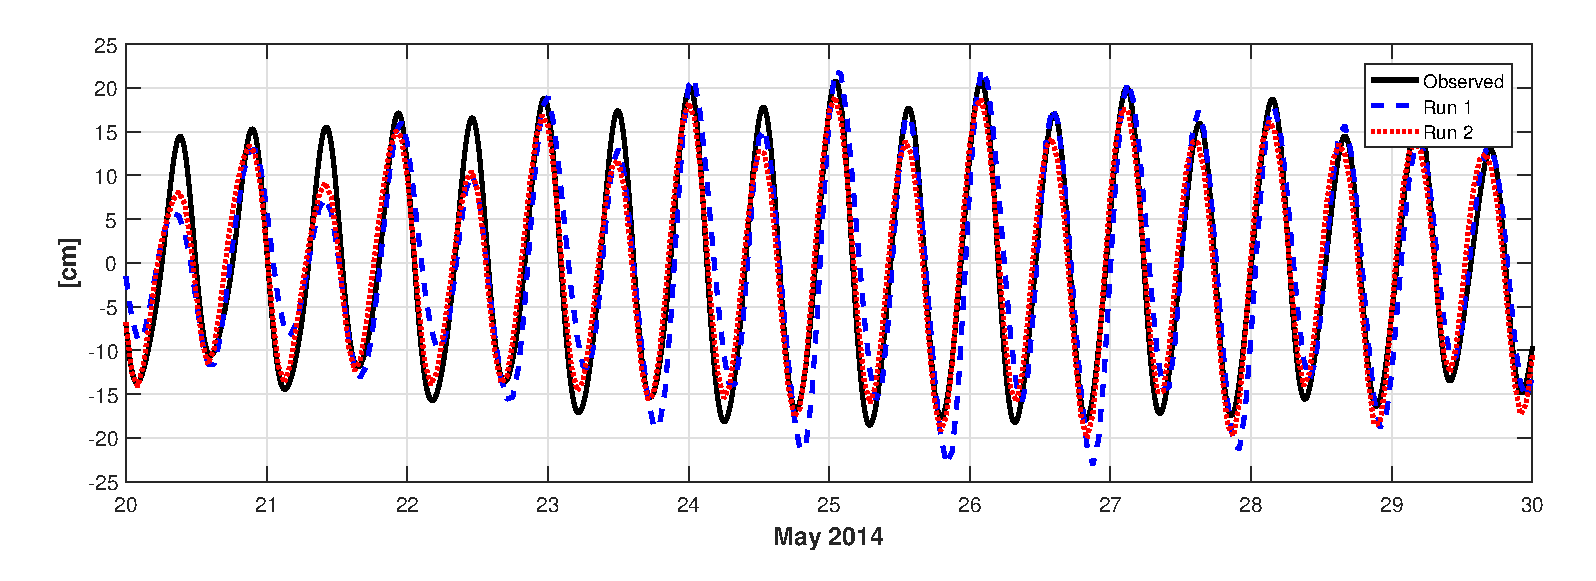
\includegraphics[width=\textwidth]{fig_Viker_timeseries}
\caption{Time series of water level at a position close to Viker}
\label{fig:Viker_timeseries}
\end{figure}



\begin{table}[ht]
%\vspace{-1.5cm}
\caption{Tidal amplitudes [cm] and phases [deg] for the water level at Viker together with adjustment factor $c$ and phase shift $\triangle \phi$ for each component}
\label{tab:Viker}
\centering
\begin{tabular}{crrrrrrrrrr} \hline
       & Period & \multicolumn{2}{c}{Observed} & \multicolumn{2}{c}{Run 1} & \multicolumn{2}{c}{Run 2} & \multicolumn{2}{c}{Adjustment} \\
Comp.  & [h] $\;\;$ & [cm] & [deg] & [cm] & [deg] & [cm] & [deg] & $c\;\;$ & $\triangle \phi$  \\ \hline 
S$_2$  &  12.0000 &   3.0 &  39 &    5.1 &  81 &    3.2 &  67 &    0.588 &   -42.4   \\
M$_2$  &  12.4206 &  11.8 & 105 &    9.7 & 122 &   11.8 & 105 &    1.224 &   -16.8   \\
N$_2$  &  12.6584 &   3.4 &  57 &    5.7 &  81 &    3.1 &  69 &    0.595 &   -24.2   \\
K$_1$  &  23.9345 &   0.7 & 136 &    1.2 & 212 &    0.1 & 198 &    0.554 &   -75.9   \\
P$_1$  &  24.0659 &   0.5 &  66 &    1.2 & 212 &    0.1 & 198 &    0.424 &  -145.5   \\
O$_1$  &  25.8193 &   2.2 & 279 &    3.7 &  19 &    2.9 & 338 &    0.591 &   259.8   \\
MN$_4$ &   6.2692 &   0.4 & 263 &    1.0 & 141 &    0.3 &   7 &    0.368 &   122.2   \\
M$_4$  &   6.2103 &   1.2 & 275 &    0.7 &  25 &    1.1 & 354 &    1.742 &   249.2   \\
MS$_4$ &   6.1033 &   0.3 & 348 &    1.1 & 111 &    0.6 &  80 &    0.272 &   236.7   \\ \hline
\end{tabular}
\end{table}


\begin{table}[ht]
%\vspace{-1.5cm}
\caption{Tidal amplitudes [cm] and phases [deg] for the water level at Oscarsborg}
\label{tab:Oscarsborg}
\centering
\begin{tabular}{crrrrrrrrrr} \hline
      & Period & \multicolumn{2}{c}{Observed} & \multicolumn{2}{c}{Run 1} & \multicolumn{2}{c}{Run 2}  \\
Comp. & [h] $\;\;$ & [cm] & [deg] & [cm] & [deg] & [cm] & [deg]  \\ \hline 
S$_2$  & 12.0000 &  3.6 &  59  &   6.1 &  85  &  3.7 &  69.8  \\
M$_2$  & 12.4206 & 13.7 & 121  &  11.1 & 128  & 13.7 & 111.0  \\
N$_2$  & 12.6584 &  3.9 &  74  &   6.6 &  86  &  3.6 &  75.1  \\
K$_1$  & 23.9345 &  0.9 & 138  &   1.1 & 213  &  0.1 &  44.1  \\
P$_1$  & 24.0659 &  0.7 &  75  &   1.1 & 213  &  0.1 &  44.1  \\
O$_1$  & 25.8193 &  2.4 & 281  &   3.9 &  21  &  3.1 & 340.2  \\
MN$_4$ &  6.2692 &  0.6 & 308  &   2.0 & 163  &  0.5 &  29.1  \\
M$_4$  &  6.2103 &  1.7 & 319  &   1.4 &  44  &  2.0 &  14.5  \\
MS$_4$ &  6.1033 &  0.4 &  32  &   2.2 & 135  &  1.3 & 105.5  \\ \hline 
\end{tabular}
\end{table}




\begin{figure}[!t]
\centering
\includegraphics[trim=1cm 1cm 0cm 0cm,clip=true,width=0.49\textwidth]{fig_Oslofjorden_M2amp.eps}
\includegraphics[trim=1cm 1cm 0cm 0cm,clip=true,width=0.49\textwidth]{fig_Oslofjorden_M2phase.eps}
%\includegraphics[width=0.33\textwidth]{fig_Oslofjorden_M2camp.eps}
\caption{Fields of M$_2$ water level amplitude and phase in the Oslofjord. The corresponding observed values are indicated by coloured circles at the three permanent gauges in the area.}
\label{fig:Oslofjord_tidal_fields}
\end{figure}


\begin{figure}[!t]
\centering
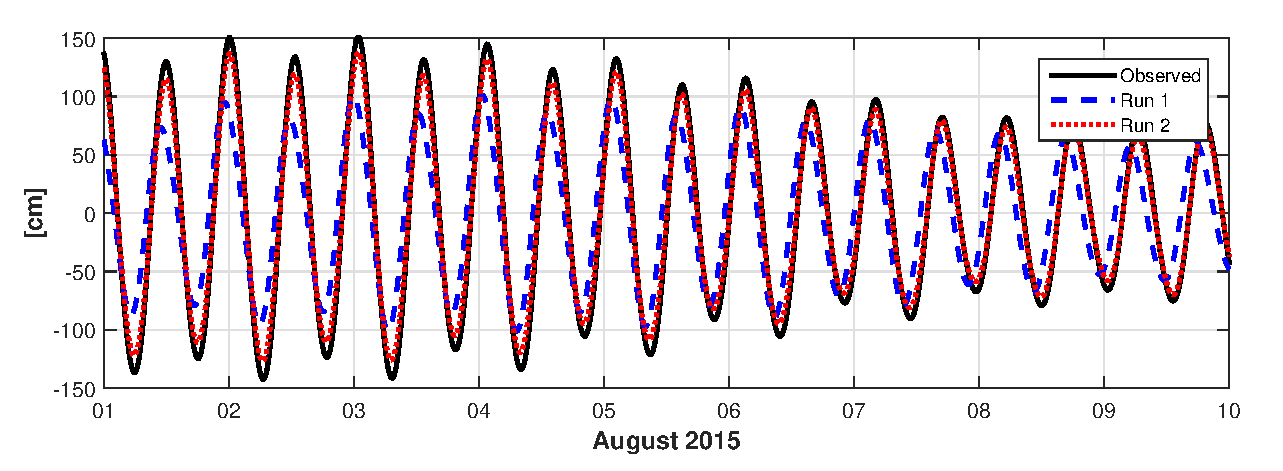
\includegraphics[width=\textwidth]{fig_Saltstraumen_timeseries}
\caption{Time series of water level at a position close to Bod{\o}}
\label{fig:Saltstraumen_timeseries}
\end{figure}


\begin{figure}[!t]
\centering
\includegraphics[width=\textwidth]{fig_Saltstraumen_M2amp}
\includegraphics[width=\textwidth]{fig_Saltstraumen_M2phase}
\caption{Fields of M$_2$ water level amplitude and phase in the Saltstarum model.}
\label{fig:Saltstraumen_field}
\end{figure}

\begin{table}[ht]
%\vspace{-1.5cm}
\caption{Tidal amplitudes [cm] and phases [deg] for the water level at Bod{\o} together with adjustment factor $c$ and phase shift $\triangle \phi$ for each component}
\label{tab:Bodo}
\centering
\begin{tabular}{crrrrrrrrrr} \hline
      & Period & \multicolumn{2}{c}{Observed} & \multicolumn{2}{c}{Run 1} & \multicolumn{2}{c}{Run 2} & \multicolumn{2}{c}{Adjustment} \\
Comp. & [h] $\;\;$ & [cm] & [deg] & [cm] & [deg] & [cm] & [deg] & $c\;\;$ & $\triangle \phi$  \\ \hline 
S$_2$   & 12.0000  &  30.0 &      8   &  19.1 &     16   &  28.1 &      7    &   1.570  &    -7.2   \\ 
M$_2$   & 12.4206  &  87.3 &    331   &  60.0 &    301   &  78.3 &    330    &   1.454  &    29.8   \\ 
N$_2$   & 12.6584  &  18.5 &    308   &  12.7 &    271   &  16.7 &    309    &   1.461  &    37.2   \\ 
K$_1$   & 23.9345  &  10.8 &    194   &   8.8 &    183   &  10.7 &    194    &   1.225  &    11.5   \\ 
O$_1$   & 25.8193  &   3.8 &     33   &   3.3 &     39   &   3.7 &     33    &   1.154  &    -6.1   \\ 
MN$_4$  &  6.2692  &   1.5 &    229   &   0.4 &    122   &   1.5 &    228    &   3.000  &   106.9   \\ 
M$_4$   &  6.2103  &   2.7 &    268   &   3.3 &    159   &   3.1 &    283    &   0.808  &   109.5   \\ 
MS$_4$  &  6.1033  &   1.3 &      2   &   1.5 &    152   &   1.4 &     30    &   0.861  &  -149.6   \\ \hline
\end{tabular}
\end{table}
